\documentclass[a4paper, 10pt]{article}
\usepackage[utf8x]{inputenc}
\usepackage{geometry}
\usepackage{graphicx}
\usepackage{amsmath}
\usepackage{amssymb}
\usepackage{mathrsfs}
\usepackage{mdwlist}
\geometry{hmargin=2.5cm, vmargin=1.5cm}

%opening
\title{GE20 - Dropbox}
\author{Pierre-François Rouleau - Antoine Hars}

\begin{document}

\maketitle

\section*{Contexte}
De nos jours, La consommation de service ne cesse de s'accro\^itre en plus de la consommation de produits issus de l'industrie.
Cette consommation croissante de services soutenue par une \'evolution constante des technologies informatiques permet aux consommateurs
de changer leurs habitudes comme dans certains cas tels que le stockage de donn\'ees.\\ \\
Nous pouvons prendre comme exemple les \'evolutions des habitudes des consommateurs pour le transfert et le transport de fichiers :
D'une utilisation de support physique de type cl\'e usb ou disque dur portable, les utilisateurs ont tendance \`a se tourner vers des solutions
ne requ\'erant aucun support physique comme le stockage en ligne sur des serveurs distants.
On utilise le terme de \textit{Cloud Computing} pour d\'esigner les techniques de sauvegarde distante de donn\'ees sur des serveurs.
En utilisant cette façon de faire, les utilisateurs du \textit{Cloud} n'ont pas \`a se soucier du support pour la sauvegarde mais
seulement des donn\'ees sauvegard\'ees.\\
Cette \'evolution dans le stockage apporte une plus grande simplicit\'e pour les utilisateurs
qui n'ont besoin que d'un ordinateur et d'une connexion internet pour receuillir leurs donn\'ees
au lieu de devoir faire attention aux diff\'erentes cl\'es usb que les consommateurs peuvent avoir.\\ \\
nous avons pu observer qu'un des services de \textit{Cloud Computing} connaissait un plus large succ\`es
que ses concurrents aupr\`es des consommateurs : Le service DropBox.
Nous avons donc choisi de nous int\'eresser et d'\'etudier ce service tout particuli\`erement.

\section*{Pr\'esentation de DropBox}

\includegraphics[height = 2cm, width = 6cm]{dropbox_logo.png}\\
DropBox est un service de stockage et de partage de fichiers en ligne permettant \`a ses utilisateurs de stocker et
de synchroniser des fichiers entre plusieurs ordinateurs.\\
Ce service s'est fait surtout connaitre du grand public par son refus de rachat
par l'entreprise Apple pour un montant de 800 millionz de Dollars.\\ \\
Ce service se veut simple d'utilisation et ce sur n'importe quelle plateforme.
Il fonctionne donc sur les syst\`emes d'exploitation Windows, Linux et Mac, ainsi que sur les appareils de type Smartphone et tablette).\\ \\
Dans le but de palier aux soucis que l'utilisation de supports physiques pouvaient engendrer (perte, oubli, etc..),
les deux fondateurs du service DropBox, Drew Houston et Arash Ferdowsi (deux anciens \'etudiants de la MIT), ont fond\'e leur startup en 2007.
Ils ont ensuite lanc\'e le d\'eploiement de leur solution de stockage en ligne courant 2008,
l'entreprise est localis\'ee \`a San Francisco en Californie.

\newpage
\noindent
DropBox a effectu\'e plusieurs acquisitions assez importantes comme :
\begin{itemize}
 \item le rachat de \textbf{Cove}, un outil puissant de collaboration dans l'\'elaboration de projets informatiques
 \item le rachat du service \textbf{AudioGalaxy} qui proposait un outil de partage de musiques
 \item le rachat de l'entreprise \textbf{Snapjoy} pour une meilleure int\'egration des photos dans le service DropBox
 \item le rachat de la startup \textbf{TapEngage} pour une gestion et un affichage efficaces des publications et des annonces
sur diff\'erentes tailles d'\'ecran.
 \item le rachat du client de messagerie \textbf{MailBox} de la compagnie Orchestra pour un montant de 100 millions de Dollars
afin de permettre de stocker des donn\'ees dans son Cloud tout en les rendant accessibles depuis son service de messagerie
(Google a le m\^eme fonctionnement avec Gmail et Google Drive, un service semblable \`a DropBox)
\end{itemize}
Ces acquisitions nous ont permis d'observer que DropBox tend \`a \^etre plus qu'un simple syst\`eme de stockage de donn\'ees en ligne,
mais souhaite proposer \`a ses clients, une solution, un service capable de g\'erer de mani\`ere simple et efficace
tous les types de fichiers courants.
Par exemple, pouvoir \'ecouter sa musique sans avoir le fichier d'une chanson sur son appareil,
pouvoir partager et surtout regarder ses photos facilement et
pouvoir d'offrir une solution g\'en\'erique permettant de g\'erer ses donn\'ees stock\'ees sur le Cloud en y associant des mails.\\ \\
En 2012, DropBox a lev\'e des fonds valorisant la soci\'et\'e \`a un montant de 4 milliards de dollars et
pr\'epare son entr\'ee en bourse pour la fin de l'ann\'ee 2013.

\section*{Le fonctionnement du service DropBox}
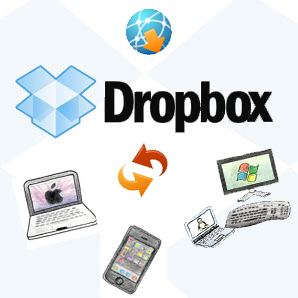
\includegraphics[height = 4cm, width = 4cm]{dropbox_1.png}
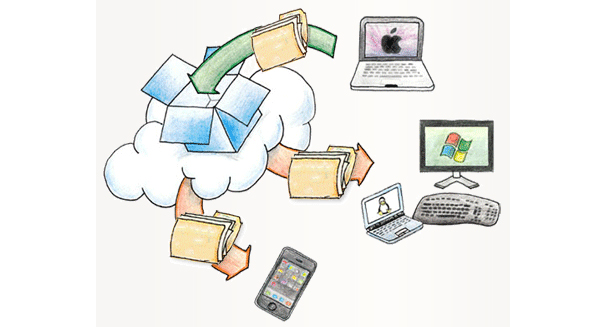
\includegraphics[height = 3cm, width = 6cm]{dropbox_3.jpg}\\
Pour permettre d'avoir acc\`es \`a ses fichiers sans support physique de type cl\'e usb, DropBox fonctionne de la mani\`ere suivante :\\
Lors de l'installation de l'application sur la machine d'un client, un agent est install\'e.
Cette agent a pour but d'envoyer chaque modification de fichier observ\'ee sur les serveurs de l'entreprise DropBox.
Une fois le fichier enregistr\'e sur un des serveurs de DropBox, il est transf\'er\'e sur toutes les machines abonn\'ees
au compte du client effectuant la manipulation.
Les agents de synchronisation de chacune des machines se chargent donc de recevoir des serveurs les modifications de fichier pour
finaliser la synchronisation des fichiers entre les diff\'erentes machines \`a disposition du client.
Nous pouvons dire que tout changement dans un dossier DropBox donne lieu \`a un \'ev\`enement qui, si le fichier est modifi\'e,
d\'eclenche une synchronisation du d\^it fichier.\\ \\
Un point important de l'utilisation d'un service de type DropBox vient du fait que les donn\'ees sont h\'eberg\'ees localement d'une part
et sur un serveur distant d'autre part (nous pouvons utiliser le terme de cloud ou nuage pour d\'efinir cette sauvegarde sur un serveur distant).
Cette sauvegarde \`a distance apporte un m\'ecanisme d'historique des modifications et donc
permet aux utilisateurs de rattraper les \'eventuelles erreurs op\'er\'ees sur leurs fichiers et
surtout les suppressions non-voulues de fichiers.\\
Gr\^ace ce service, il n'est plus question de se soucier de l'utilisation d'un support physique pour transporter ses donn\'ees
ou de l'utilisation des envois de fichiers par email pour r\'ecup\'erer ses donn\'ees.\\
Concernant la s\'ecurit\'e dans le stockage des donn\'ees, les communications pour la synchronisation des fichiers est crypt\'ees et
les dossiers priv\'es sont eux aussi crypt\'es. Ils ne sont accessibles que par les personnes que le client ont invit\'e.

\newpage

\section*{Les statistiques}
Dans un secteur o\`u la comp\'etition est rude avec beaucoup de concurrence (on a d\'enombr\'e une vingtaine d'applications de stockage en ligne)
DropBox a su cro\^itre tr\`es rapidement :
Fin 2008, ce service comptabilisait un total de 100 000 utilisateurs diff\'erents.
En 2009, il en comptait 2 millions, 4 millions en 2010, 25 millions en 2011 et
\`a la fin 2012, l'entreprise comptabilisait 100 millions de clients diff\'erents.\\
L'application est install\'ee sur pas moins de 250 millions d'appareils et
en terme de fichier, 1 milliards de fichiers sont sauvegard\'es tous les 48 heures.\\
Du point de vue financier, DropBox comptabilise une centaine d'employ\'es et g\'en\'erait des revenus \`a hauteur
de 240 millions de Dollars en 2011.

\section*{L'\'economie associ\'ee \`a DropBox}
Dropbox est d\'ecoup\'ee en 2 sections pour appliquer le mod\`ele \'economique Freemium:
\begin{itemize*}
 \item Une offre gratuite de base.
 \item Une offre premium payante.
\end{itemize*}
Les clients se voient offrir un compte gratuit lors de l'inscription avec un espace de stockage limit\'e \`a 2 Go.
Pour b\'en\'eficier de plus d'espace de stockage, les clients ont plusieurs possibilit\'es :
\begin{itemize*}
 \item parrainer de futurs clients en fournissant un lien sp\'ecial d'inscription.
\`A chaque fois qu'un nouvel utilisateur s'inscrit en utilisant ce lien, 500 Mo sont ajout\'es au compte parrain.
Au total, il est possible de parrainer 32 amis pour obtenir de l'espace de stockage ce qui correspond \`a 16 Go.
 \item se connecter aux r\'eseaux sociaux (Facebook et Twitter).
 \item donner son avis sur le service DropBox.
 \item ex\'ecuter toutes les \'etapes de prise en main du service DropBox.
 \item basculer son compte gratuit en compte premium payant qui nous permet d'ajouter un espace de 100 Go, ou 200 Go ou encore 500 Go.
 \item basculer son compte gratuit en compte entreprise qui se tourne vers les entreprises d\'esirant int\'egrer le \textit{Cloud Computing}
dans leurs processus de production. Dans ce cas de figure, la taille de l'espace de stockage n'est plus le point primordial de l'offre mais
plut\^ot le nombre de personnes qui interagissent en m\^eme temps sur le projet. Le service DropBox pour ce cas, offre une plus forte s\'ecurit\'e,
un support t\'el\'ephonique et les outils n\'ecessaires pour la gestion des versions d'application.
\end{itemize*}

\section*{La r\'eussite de DropBox}
Du fait de sa simplicit\'e d'utilisation, DropBox se d\'emarque de ses concurrents et
a atteint 50 millions de clients actifs en seulement quelques ann\'ees.
De plus, 96\% de ses utilisateurs poss\`edent un compte classique (non payant).\\
L'impressionnante r\'eussite de DropBox par rapport \`a ses concurrents vient du fait que dans un premier temps,
qu'il s'agit d'un service simple et disponible sur toutes les plateformes du march\'e et
que dans un second temps, ce service dispose d'une communaut\'ee d'utilisateurs tr\`es pr\'esente et soucieuse
de contribuer \`a l'am\'elioration du produit.\\
DropBox a su imposer un service, non primordial pour les consommateurs en amont, devenu indispensable par la suite pour ces clients,
les risques \'etant de proposer un produit qui n'int\'eresserait personne.\\
Avant l'arriv\'ee de DropBox sur le march\'e, les syst\`emes de stockage et de partage de fichiers en ligne avaient d\'ej\`a \'et\'e mis en place
mais aucun n'avait su s'imposer aupr\`es du grand public car ne proposant pas un produit simple et utilisable sur tous les supports disponibles.\\
Ces syst\`emes \'etaient plut\^ot utilis\'es par des utilisateurs aguerris et non novices.\\ \\
Il est important de notifier que tr\`es peu d'annonces publicitaires ont \'et\'e effectu\'ees pour promouvoir ce service,
la promotion de DropBox n'a eu lieu que par l'interm\'ediaire de ses clients au moyen du bouche-\`a-oreille et du parrainage principalement.\\ \\
Tout au long de son processus d'am\'elioration de la qualit\'e de son produit, DropBox a laiss\'e une place primordiale aux retours de ses clients
(il est possible de gagner de l'espace de stockage en envoyant une critique du service \`a l'entreprise).
L


\section*{Probl\'ematique}
Dans un contexte o\`u la concurrence est tr\`es pr\'esente, quels ont \'et\'e les outils qui ont permis la r\'eussite de ce service
cr\'e\'e \`a la base par des ing\'enieurs non expert en marketing ?\\
Suivant


\end{document}
